\chapter{Probabilità}
Il calcolo delle probabilità è una teoria della matematica che permette di descrivere e studiare \underline{Fenomeni Aleatori}.
\\Un \textbf{Fenomeno Aleaotrio} (o casuale) é un fenomeno il cui esito \emph{non è prevedibile con certezza} a priori.
\section{Assiomi della Probabilità}
La probabilitá si basa sullo studio di \textbf{Esperimenti Aleatori}, ovvero esperimenti il cui risultto non è prevedibile con certezza.
Per poter studiare gli eseprimenti aleatori bisogna poterli descrivere matematicamente. 
La loro descrizione matematica si articola in tre passi:
\begin{enumerate}
    \item \textbf{Spazio campionario} (o spazio degli esiti)
    \\ $\to$ Insieme $\Omega$ che contiene tutti i possibili esiti dell'esperimento 
    \\ \small{es. Tiro un dado a sei facce $\Omega = {1, 2, 3, 4, 5, 6}$}
    \item \textbf{Eventi}
    \\ $\to$ I sottinsiemi dello spazio campionario $A \subseteq \Omega$ che riassumono affermazioni sull'esito dell'esperimento aleatorio.
    \\ \small{es. Tiro un dado a sei facce: esce un numero pari $A = {2, 4, 6}$}
    \item \textbf{Probabilità}
    \\ $\to$ Regola che assegna, in modo coerente, a ogni evento $A \subseteq \Omega$ un "\textbf{grado di fiducia}" $P(A)$, tra 0 e 1, che attribuiamo al verificarsi di A.
\end{enumerate}
Matematicamente la \textbf{Probabilità} é una funzione $P:\rho(\Omega) \to [0,1]$ che soddisfa opportune proprietá.
In questo caso $\rho(\Omega)$ sono tutti i sottoinsiemi di $\Omega$.

\subsection*{Operazioni insiemistiche e Logiche}
Nella definizione degli eventi, che sono concetti logici tradotti in concetti insiemistici, ci sono dei parallelismi tra le operazioni logiche e quelle insiemistiche:
\begin{itemize}
    \item Unione $A\cup B$ $\longleftrightarrow$ Si verifica $A$ o $B$ o entrambi.
    \item Intersezione $A \cap B$ $\longleftrightarrow$ Si verificano $A$ e $B$.
    \item Complementare $A^c$ $\longleftrightarrow$ Non si verifica $A$.
\end{itemize}
Ci sono poi anche due interessanti proprietá dei complementari:
\begin{itemize}
    \item $(A^c)^c = A$ (doppia negazione)
    \item Leggi di Demorgan: $(A \cup B)^c = A^c \cap B^c$ e $(A \cap B)^c = A^c \cup B^c$
\end{itemize}

\subsection{Interpretazioni di $P(A)$}
Che cosa significa grado di fiducia? cosé $P(A)$?
\\Esistono due diverse interpretazioni sul grado di fiducia, entrambe equamente valide:
\paragraph{Interpretazione Soggettivista} In questa interpretazione $P(A)$ é il prezzo equo di una scommessa che paga 1 se si 
verifica $A$ e 0 altrimenti.
\paragraph{Intrepretazione Frequentista} In questa interpretazione invece $P(A)$ è la frazione asintotica di volte in cui si verifica $A$ ripetendo l'esperimento.

\paragraph*{}Quale scelgo? Entrambe queste interpretazioni sono valide, quindi si puó scegliere quella che si vuole.
Tutte e due queste interpretazioni peró devono soddisfare le due Proprietà di Base.

\section{Proprietà di base} 
Ogni interpretazione probabilistica deve rispettare queste due proprietà fondamentali:
\begin{enumerate}
    \item $P(\Omega) = 1$, ovvero la probabilitá dello spazio campionario deve essere 1 (massima).
    \item Se A e B sono eventi disgiunti, cioè $A \cap B \neq \emptyset$, allora deve valere che $P (A \cup B) = P(A) + P(B)$
\end{enumerate}
Da queste proprietá si deriva la Definizione dell'approccio moderno alla probabilitá, definito da Kolmogorov nel 1933:
\definizione{
    Sia $\Omega$ un insieme (spazio campionario).
    Si dice \textbf{Probabilità} qualsiasi funzione $P:\rho(\Omega) \to [0,1]$ che soddisfa:
    \begin{enumerate}
        \item $P(\Omega)= 1$
        \item Se $A\cap B = \emptyset \implies P(A \cup B) = P(A) + P(B)$.
    \end{enumerate}
    La coppia $(\Omega, P)$ é detta \textbf{Spazio di Probabilità}
}

\paragraph{La coppia $(\Omega, P)$ è detta \textbf{Spazio di Probabilità}}.
\\ Fissiamo uno spazio di probabilità $(\Omega, P)$.
Da queste proprietà si deducono molte altre proprietà
\begin{itemize}
    \item $P(\emptyset) = 0$
    \item \textbf{Regola del complementare} $\to P(A^c) = 1 - P(A)$ \\ Vale per ogni A
    \item \textbf{Regola della addizione di probabilità} $\to P(A \cup B) = P(A) + P(B) - P(A \cap B)$ 
    \\ Vale per ogni A, B (anche $A \cap B \neq \emptyset$)
    \item Monotonia: se $A \subseteq B$ allora $P(A) <= P(B)$
\end{itemize}
\paragraph{Analogia} c'è un analogia tra probabilità e area
\begin{center}
    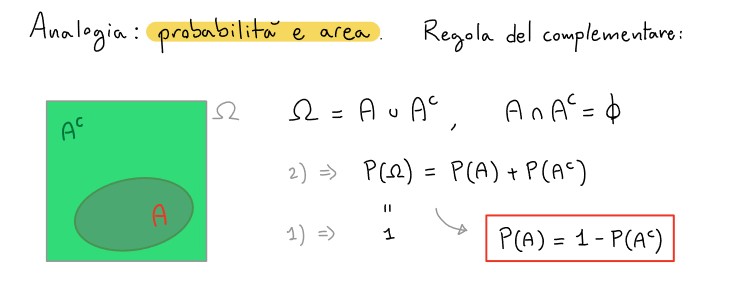
\includegraphics[width=120mm,scale=0.5]{analogia_prob_area.png}
\end{center}



\section{Calcolo combinatorio}
Consideriamo uno spazio di probabilità uniforme $(\Omega, P)$
\begin{itemize}
    \item $P(A) = \frac{|A|}{|\Omega|}$ = $\frac{Casi favorevoli}{Casi Possibili}$
    per ogni $A \subseteq \Omega$
    \item $P({w}) = \frac{1}{\Omega} = \frac{1}{n}$ per ogni $w \in \Omega$
\end{itemize}
Questo è il modello appropriato per descrivere esperimenti aleatori i cui esiti
siano tutti equiprobabili. Quando scegliamo casualmente una persona/oggetto in un 
insieme finito senza ulteriori specifiche, si sottintende che la scelta è effettuata
in modo uniforme.
Affinchè la probabilità uniforme sia ben definita, lo spazio campionario $\Omega$
deve essere finito (se così non fosse la probabilità uniforme su $\Omega$ non esiste)
\\ In uno spazio di probabilità uniforme calcolare una probabilità significa contare gli 
elementi di un insieme
\begin{equation}
    P(A) = \frac{|A|}{|\Omega|}
\end{equation}
Dato che contare non è banale per insiemi grandi sono nate tecniche di conteggio,
esse formano il \textbf{Calcolo Combinatorio}
\paragraph{Principio Fondamentale} Consideriamo un esperimento costituito da due parti:
\begin{enumerate}
    \item n esiti possibili
    \item m esiti possibili
\end{enumerate}
L'esperimento totale può avere $n*m$ esiti possibili.
\paragraph{Esempio} Il lancio dei dadi. Se lancio 2 dadi a sei facce ho $\Omega$ 
esiti possibili
\begin{equation}
    |\Omega| = 6*6 = 36
\end{equation}
\subsection{Disposizioni con ripetizione}
Sequenze ordinate di k elementi (anche ripetuti) scelti tra n possibili. Numero totale è:
\begin{equation}
    n*n \dots n = n^k
\end{equation}
\paragraph{Esempio} Estrazione casuale di 3 persone, calcolare la probabilità che
siano tutte nate in primavera.
In questo caso lo spazio campionario sono i compleanni delle tre persone quindi
\begin{equation}
    \Omega = {(x_1, x_2, x_3): x_1, x_2, x_3 \text{ in Calendario}}
\end{equation}
Questa è una disposizione con ripetizione di 3 elementi estratti dal calendario
\begin{equation}
    |\Omega| = 365*365*365 = 365^3
\end{equation}
Probabilità uniforme $P(A) = \frac{|A|}{|\Omega|}$
\\ In questo caso tutti i nati in primavera vengono considerati 
nati A = tutti  nati in primavera = [20 marzo, 21 giugno) e in totale sono 92 giorni.
\\ Si tratta anche qua di una disposizione ripetuta di 3 elementi.
\begin{equation}
    |A| = 92*92*92 = 92^3
\end{equation}
Per calcolare la probabilità è sufficiente dividere A per $\Omega$
\begin{equation}
    P(A) = \frac{|A|}{|\Omega|} = \frac{92^3}{365^3} = 0,016 = 1,6\%
\end{equation}
Se avessi estratto k persone sarebbe stato sufficiente sostituire l'esponente con k.

\subsection{Disposizioni semplici}
Sequenze ordinate di k elementi distinti scelti tra n possibili (con $k <= n$) 
\textbf{senza ripetizione}
\begin{equation}
    n*(n-1)*(n-2)\dots(n-k+1) = \frac{n!}{(n-k)!}
\end{equation}
\'E preferibile utilizzare la prima formula su R dato che il fattoriale scala molto male,
su carta spesso si semplifica, ma su Computer si calcolerebbe tutto il fattoriale e spesso richiede 
molto tempo.
\\ Se $k = n$ si parla di \textbf{Permutazioni} di n oggetti. In numero sono:
\begin{equation}
    n! = n*(n-1)*(n-2)\dots 2 * 1
\end{equation}
\paragraph{Esempio}. Quanti sono i possibili ordini di arrivo di 3 squadre?
Si tratta di una permutazione di 3 elementi.
\paragraph{Esempio Paradosso dei compleanni}

\subsection{Combinazioni}
In molti casi non siamo interessati all'ordine. 
Per esempio, se dobbiamo scegliere un comitato di 2 persone non ci interessa l'ordine 
dei candidati.
Si parla in questo caso di combinazioni, esse si possono ottenere dalle disposizioni semplici
"dimenticando" l'ordine degli elementi.
\begin{equation}
    {n \choose x} = \frac{n!}{k!(n-k)!}
\end{equation}
Insiemi = collezioni (non ordinate) di k elementi distinti scelti tra n possibili (con $k <= n$).
\paragraph{Esempio}. Mano di carte a Poker, un giocatore riceve 5 carte estratte da un mazzo che
ne contiene 52. Il numero di possibili mani è
\begin{equation}
    {52 \choose 5} = \frac{52!}{5!47!}
\end{equation} 

\section{Probabilità Condizionata}
Consideriamo un esperimento aleatorio, che descriviamo con uno spazio di probabilità $(\Omega, P)$.
Consideriamo un evento $A \subseteq \Omega$, che ha un probabilità $P(A)$.
Supponiamo di ricevere l'informazione che un altro evento B si è verificato.
Come è ragionevole aggiornare la probabilità di A per tenere conto di questa informazione aggiuntiva?
\\La soluzione è data dalla probabilità Condizionata.
\begin{equation}
    P(A|B) = \frac{P(A \cap B)}{P(B)}
\end{equation}
La precedente formula denota la probabilità condizionata di A dato B (o sapendo B).
Sto quindi calcolando la probabilità di A.
\begin{center}
    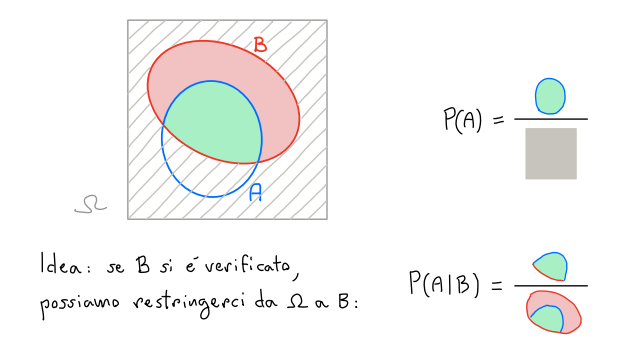
\includegraphics[width=120mm,scale=0.5]{prob_condizionata_area.png}    
\end{center}
Quando si verifica un evento lo spazio di probabilità si riduce (vedere esempio sui dadi)
\subsection{Regola del prodotto}
\begin{equation}
    P(A \cap B) = P(A)*P(B|A)
\end{equation}
\subsection{Formula di Disintegrazione}
\begin{equation}
    P(A) = P(A \cap B) + P(A \cap B^c)
\end{equation}
\subsection{Formula delle probabilità totali}
\begin{equation}
    P(A) = P(A|B)P(B) + P(A|B^c)P(B^c)
\end{equation}
Inoltre $P(*|B)$ + una probabilità, in particolare:
\begin{equation}
    P(A^c|B) = 1 - P(A|B)
\end{equation}
\subsection{Formula di Bayes}
\begin{equation}
    P(B|A) = \frac{P(A|B)P(B)}{P(A)}
\end{equation}
\paragraph{Esempio}. Per vedere la parte pratica andare a vedere l'esempio sui tamponi
per rilveare la presenza di un virus. Super interessante e utile.
\\Il file è \textbf{Appunti Lezione 3 - In fondo al PDF}

\section{Indipendenza di eventi}
Può capitare che, per un evento A, l'informazione che un altro evento B si è verificato
non ne cambi la probabilità.
\begin{equation}
    P(A|B) = P(A)
\end{equation}
che equivale
\begin{equation}
    P(A \cap B) = P(A)P(B)
\end{equation}
In questo caso gli eventi A e B si dicono \textbf{Indipendenti}
\paragraph{Esempi}
Lancio di due dadi, i risultati sono eventi indipendenti
\\ Urna contenente 5 palline rosse e 3 palline verdi. Pesco in successione due palline, 
senza reimmissione. La probabilità che la prima pallina sia rossa e che la seconda sia rossa
sono \textbf{dipendenti}!

\subsection{Eventi indipendenti != Eventi disgiunti!}
\begin{center}
    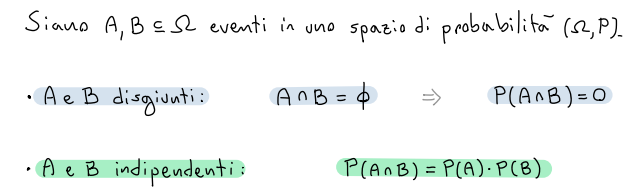
\includegraphics[width=120mm, scale=0.5]{differenza_disgiunti_indipendenti.png}
\end{center}
Quindi due eventi indipendenti non possono essere disgiunti,
tranne nel caso "banale" in cui uno dei due abbia probabilità
nulla.

\paragraph*{Esempio} Una famiglia ha due figli/e descritti da 
\\ $\Omega = \{MM, FF, FM, FF\}$ e $P=\text{Probabilità uniforme} = \frac{1}{4}$
\\ Consideriamo gli eventi:
\begin{itemize}
    \item A := "il primo genito è maschio" = \{MM, FF\}
    \item B := "il secondo genito è maschio" = \{MM, FM\}
    \item C := "la primogenita è femmina" =\{FM, FF\}
\end{itemize}
\begin{center}
    In questo caso A e B sono \textbf{indipendenti}, ma \textbf{NON disgiunti};
\\ A e C sono \textbf{disgiunti}, ma \textbf{NON indipendenti}.
\end{center}

\paragraph{Estensioni}
Tre eventi A, B, C si dicono indipendenti se valgono
\begin{center}
    $P(A \cap B \cap C) = P(A)P(B)P(C)$
    \\$P(A \cap B) = P(A)P(B)$
    \\$P(B \cap C) = P(B)P(C)$
    \\$P(A \cap C) = P(A)P(C)$
\end{center}
